\chapter{Introduction}



%\marginpar[Margin note.]{Margin par.}



\section{Overview} 

The appearance of a 3D scene refers to the visual characteristics that result from the interaction of light with materials, textures, and geometry, determining how objects are perceived in terms of colour, shading, and surface detail. It is influenced by factors such as lighting conditions, material properties, and environmental effects, which together define the realism and aesthetic quality of the rendered scene.


The appearance of a 3D scene refers to the visual characteristics and perception of objects within the scene, shaped by their interaction with light and surface properties. In the field of computer graphics and 3D rendering, the appearance is determined by several critical factors:

Lighting: The type, placement, intensity, and color of light sources define how objects are illuminated, generating shadows, highlights, and overall contrast. These lighting conditions significantly influence depth, mood, and the spatial relationships between objects.

Materials and Shaders: Materials describe the optical properties of objects, such as color, transparency, reflectivity, and surface roughness. Shaders are algorithms used to simulate these properties and determine how light interacts with the material, impacting the realism and visual complexity of the scene.

Textures: Textures are 2D images or procedural patterns applied to 3D surfaces, providing detailed surface information, such as color, bumpiness, or imperfections. They play a crucial role in simulating real-world surfaces and adding visual complexity.

Geometry and Shape: The 3D models' geometric detail and surface topology affect how light interacts with objects. More complex geometries produce varied lighting effects, such as shadows and reflections, impacting the overall visual fidelity of the scene.

Environmental Effects: Atmospheric conditions such as fog, reflections, and global illumination contribute to the overall appearance by simulating real-world environmental factors. These effects add depth and realism, influencing how the scene's objects are perceived.

Camera and Viewpoint: The position and properties of the virtual camera, including focal length and field of view, influence the composition, perspective, and the visual hierarchy of objects in the scene.

In summary, the appearance of a 3D scene is a result of the interplay between light, material properties, surface detail, and environmental factors, all of which contribute to the perceptual qualities and realism of the rendered image.



Appearance manipulation refers to the modification of visual features in images or videos, such as changing facial expressions, altering physical attributes, or transforming entire scenes. The motivations behind appearance manipulation are varied, ranging from artistic expression to functional applications. In creative industries, altering visual aesthetics allows artists, designers, and filmmakers to bring new, imaginative ideas to life. In entertainment, it enables actors to take on diverse roles or experience transformations without the need for physical makeup or prosthetics. Social media users often employ these techniques to enhance their appearance, explore identity, or simply engage in self-expression.

Applications

Appearance manipulations have wide-ranging applications across multiple fields:

Entertainment and Media: In films, video games, and virtual reality, appearance manipulation helps create convincing special effects, digitally age or de-age actors, or generate entire digital characters. In post-production, filmmakers can make subtle changes to lighting, costumes, and even an actor’s appearance to fit the tone or story.

Augmented and Virtual Reality (AR/VR): In AR/VR platforms, manipulating appearances allows users to embody avatars that differ from their real-world identities, enhancing the immersive experience. This can include changing hairstyles, outfits, or even body types.

Social Media and Advertising: Filters, face-tuning, and other aesthetic tools are now common in social media apps, allowing users to modify their appearances to align with social or aesthetic trends. In advertising, brands use manipulated visuals to create idealized product images and promotional material.

Healthcare and Surgery: In medicine, appearance manipulation helps simulate cosmetic or reconstructive surgery outcomes. Patients can see what they might look like post-procedure, aiding them in making informed decisions.

Fashion and E-commerce: Virtual try-ons for clothing and accessories allow customers to visualize how products will look on them, revolutionizing online shopping by reducing uncertainties around fit and style.

Cultural and Heritage Preservation: Digitally restoring or manipulating historical figures or scenes can bring history to life in documentaries or museums, helping people experience the past in a visually engaging manner.

One famous example from filmmaking where producers had to wait an extended period to capture a specific scene is from the movie "Boyhood" (2014), directed by Richard Linklater.

The movie was filmed over 12 years, from 2002 to 2013, as it follows the life of a young boy, Mason, from childhood to adulthood. Instead of using makeup, aging effects, or casting different actors for different stages of the character’s life, Linklater and his team waited for the actors to age naturally. Every year, the cast and crew would reunite to shoot scenes reflecting the characters' development over time.

\begin{figure}[ht]
  \centering
  % \fbox{\rule{0pt}{2in} \rule{0.9\linewidth}{0pt}}

    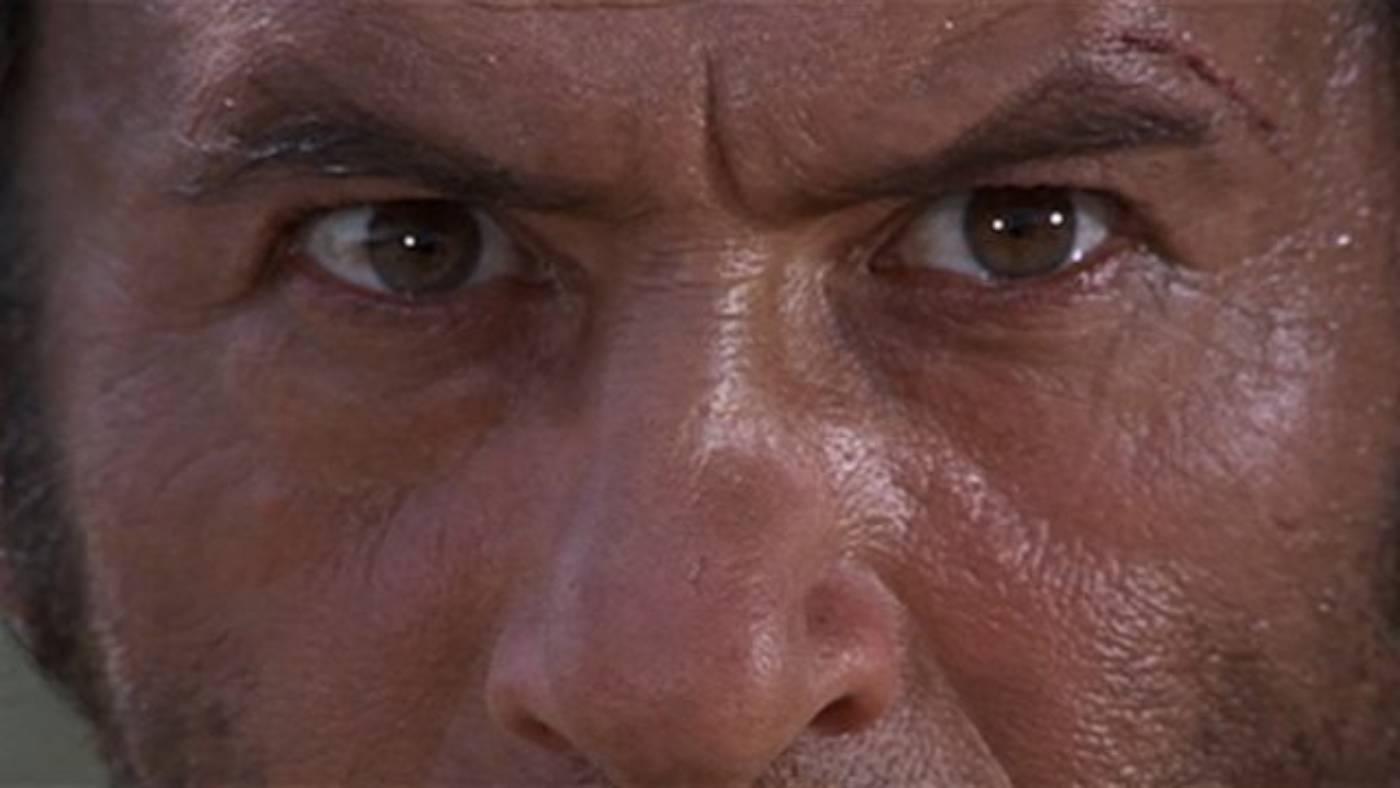
\includegraphics[width=\linewidth]{Images/A scene from ‘The Good, the Bad and the Ugly’ (1966). Image courtesy- Produzioni Europee Associati .jpg}

   \caption{A pixel, a picture element, is the smallest unit of a rendered image. Displaying an image with fewer pixels causes losses in details as one pixel starts covering a larger area in the 3D scene.}
   \label{fig:colour-approximate}
\end{figure}


\begin{wrapfigure}{r}{5cm}
  \centering
  % \fbox{\rule{0pt}{2in} \rule{0.9\linewidth}{0pt}}
   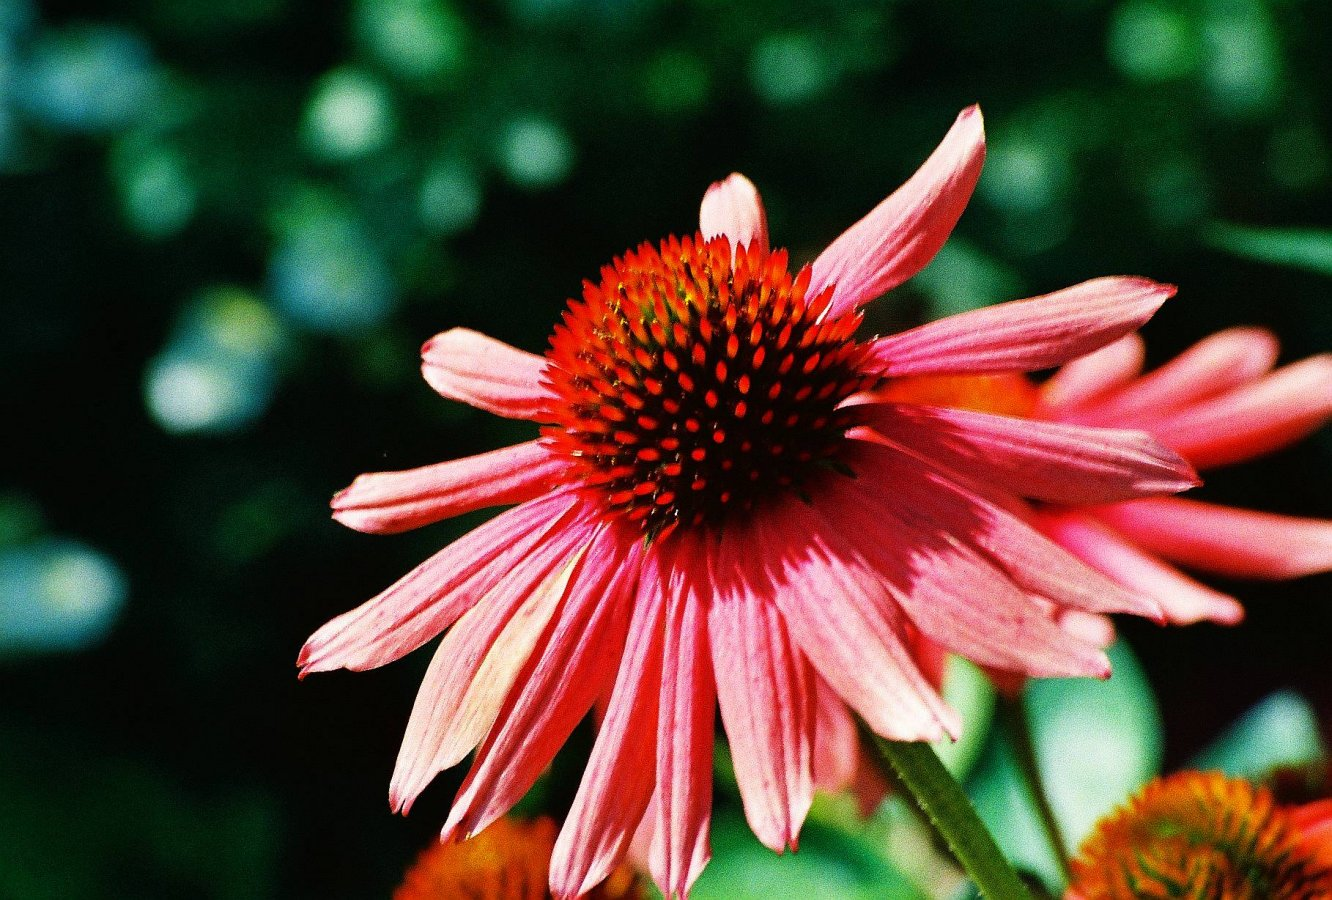
\includegraphics[width=\linewidth]{Images/byRickJones .jpg}
   
   \caption{Graph representation of a linear equation. Figure from [Issac, 2018].}
   \label{fig:neuron}
\end{wrapfigure}


\begin{figure}[ht]
  \centering
  % \fbox{\rule{0pt}{2in} \rule{0.9\linewidth}{0pt}}

    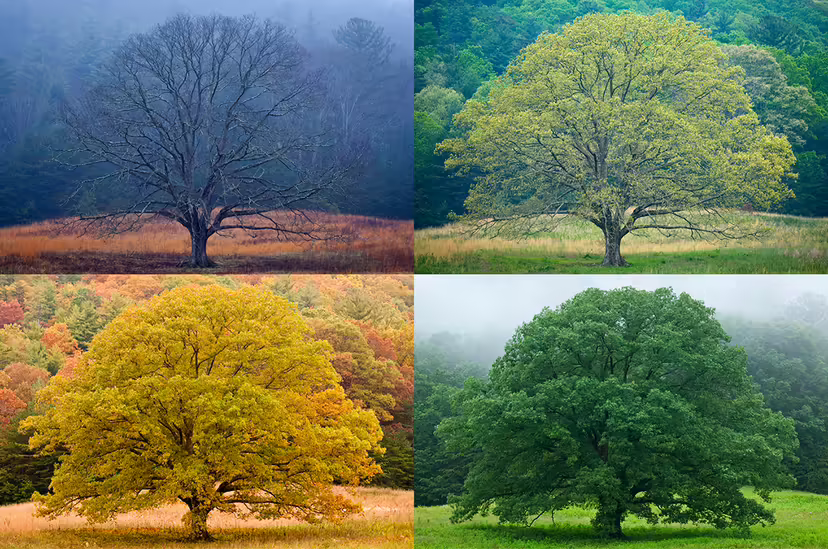
\includegraphics[width=\linewidth]{Images/seasonchanges.png}

   \caption{A pixel, a picture element, is the smallest unit of a rendered image. Displaying an image with fewer pixels causes losses in details as one pixel starts covering a larger area in the 3D scene. Image from [Michael Melford/Getty Images]}
   \label{fig:colour-approximate}
\end{figure}



\begin{figure}[ht]
  \centering
  % \fbox{\rule{0pt}{2in} \rule{0.9\linewidth}{0pt}}

    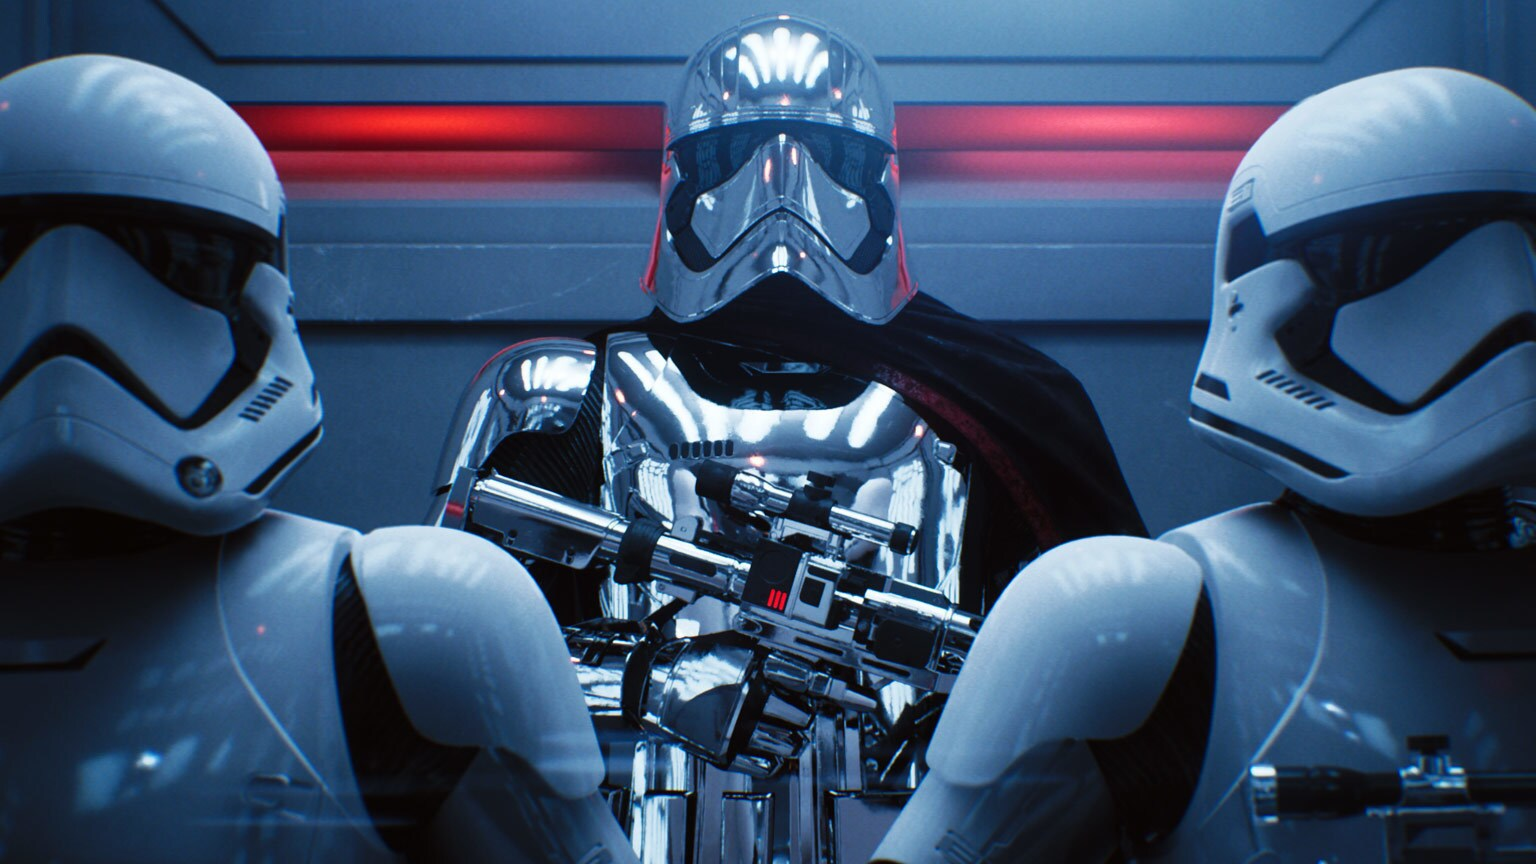
\includegraphics[width=\linewidth]{Images/StarWars-RayTracing.jpeg}

   \caption{Photorealistic rendering can be achieved through extensive ray tracing for which reflectance should be accurately measured and represented.}
   \label{fig:colour-approximate}
\end{figure}

Necessity of AI in Appearance Manipulation

AI plays a crucial role in advancing appearance manipulation due to the complexity and scale of the transformations involved. Traditional editing tools require significant time and skill, but AI-driven techniques streamline the process by automating and enhancing image and video manipulation tasks. AI algorithms can analyze and modify appearances in real time, understanding facial structures, lighting, textures, and motion.

Key contributions of AI include:

Deep Learning: Techniques such as Generative Adversarial Networks (GANs) have revolutionized appearance manipulation by generating high-quality, realistic images from data inputs. For example, GANs can create entirely new faces, alter facial expressions, or simulate aging with stunning accuracy.

Real-Time Adjustments: AI-driven filters on social media can make immediate alterations to a user’s appearance, such as changing hair color or smoothing skin, without needing manual intervention.

Customization and Scalability: AI allows for highly personalized manipulations, from altering subtle features like eye shape to transforming entire body proportions. Additionally, AI can handle large volumes of data, making it possible to apply these manipulations to millions of users simultaneously in applications like social media or AR.

Conclusion

Appearance manipulation has become an indispensable tool in modern visual culture, driving innovation in entertainment, healthcare, and beyond. AI's involvement enhances the accuracy, scalability, and creativity of appearance modifications, pushing the boundaries of what is visually possible and enabling more seamless and engaging user experiences across industries.




\section{Contributions}
\section{Publications}

The following works are produced throughout my doctoral studies and contributed to main chapters of this dissertation:

\begin{itemize}

\item \textbf{Fazilet Gokbudak}, Alejandro Sztrajman, Chenliang Zhou,  Fangcheng Zhong, Rafal Mantiuk, and Cengiz Oztireli. Hypernetworks for Generalizable BRDF Representation. \textit{ECCV 2024}

\item \textbf{Fazilet Gokbudak} and Cengiz Oztireli. Text-guided Transient Attribute Transfer. \textit{Under review}.

\item \textbf{Fazilet Gokbudak} and Cengiz Oztireli. One-shot Detail Retouching with Patch Space Neural Transformation Blending. \textit{In Proceedings of the 20th ACM SIGGRAPH European Conference on Visual Media Production (CVMP '23)}, 2023. Association for Computing Machinery, New York, NY, USA, Article 2, 1–10. https://doi.org/10.1145/3626495.3626499

\end{itemize}

The following works did not directly contribute to this dissertation; however, they helped me build skills and knowledge for the success of the main contributions:

\begin{itemize}

\item Madeleine Darbyshire, Shaun Coutts, Eleanor Hammond, \textbf{Fazilet Gokbudak}, Cengiz Oztireli, Petra Bosilj, Junfeng Gao, Elizabeth Sklar, and Simon Parsons. Multispectral Fine-Grained Classification of Blackgrass in Wheat and Barley Crops. \textit{Under Review}, 2024.

\item Chenliang Zhou, Alejandro Sztrajman, Rainer Gilles, and Fangcheng Zhong, \textbf{Fazilet Gokbudak}, Zhilin Guo, Weihao Xia, Rafal Mantiuk, and Cengiz Oztireli. Physically Based Neural Bidirectional Reflectance Distribution Function. \textit{Under Review}, 2024.

\end{itemize}

Furthermore, the work I completed during my internship at Amazon 